\documentclass[11pt]{article}

\title{{\Large Team Amalgam} \\ SE390 Requirements Specification}
\author{Joseph Hong, Chris Kleynhans, Ming-Ho Yee, Atulan Zaman \\
        \{yshong,cpkleynh,m5yee,a3zaman\}@uwaterloo.ca}

\usepackage[T1]{fontenc}
\usepackage[utf8]{inputenc}
\usepackage{ae,aecompl}

% For definitions
\usepackage{amsthm}
\theoremstyle{definition}
\newtheorem{mydef}{Definition}

\usepackage[%
  style=ieee,
  sorting=none,
  dateabbrev=false,
  backend=biber%
]{biblatex}
\addbibresource{main.bib}

% TikZ is what lets us draw graphics
\usepackage{tikz}
\usetikzlibrary{shapes.multipart,positioning,arrows}

\begin{document}
\maketitle

\begin{abstract}
Our project is to build Moolloy version 0.3. It must meet the same
functional requirements as Moolloy 0.2. In addition, Moolloy 0.3 will
improve the speed and scalability of Moolloy 0.2.
\end{abstract}

\tableofcontents
\newpage

%%%%%%%%%%%%%%%%%%%%%%%%%%%%%%%%%%%%%%%%%%%%%%%%%%%%%%%%%%%%%%%%%%%%%%
\section{Introduction}\label{sec:intro}
\subsection{Purpose}\label{sec:purpose}
% Purpose of the document
% Who is intended audience?
% How is it to be used?
% .25-.5 pages

This document is the requirements specification for Moolloy version
0.3, a computer-based system that will be developed by Team Amalgam.
This system will be developed over the course of the fourth-year design
project, which consists of the courses SE390, SE490, and SE491.

Furthermore, as the system is built on top of Moolloy, the scope of
this document includes the requirements specification for Moolloy.
The intended audience for this document will be researchers interested
in the \textit{guided improvement algorithm} for multi-objective
optimization, or any other relational logic optimization problems.

Because our work is to improve speed and
scalability---nonfunctional requirements---this expanded requirements
specification will also describe the implementation details for the
guided improvement algorithm. This background will be necessary in
order to understand our work.

Due to the fact that this is a research project and that we do not know
which optimization techniques will be implemented, this requirements
specification is subject to change. Specifically, more command-line
arguments may be added to control optimization parameters.

This document allows us, and any other researchers, to develop
benchmarks and tests for Moolloy. Furthermore, interested researchers
may also use this document to write extensions and modify the software.

\subsection{Scope}\label{sec:scope}
% Name of the software product
% Overview of the product - what it will/ will not do
% Summary of the application of the software, including benefits
% and goals
% The boundaries of the product
% .25-.5 pages

The software product described in this document will be referred to as
\textit{Moolloy v0.3}, or \textit{Moolloy} for short. Henceforth, any
references to the existing Moolloy versions will be referred to with
their version numbers, or as the \textit{original Moolloy}.

Moolloy is an implementation of the \textit{guided improvement
algorithm}, which produces Pareto-optimal solutions to general
multi-objective optimization problems. Although Moolloy is built on top
of a SAT solver, it is not a SAT solver.

Multi-objective optimization is an interest to many fields of science
and engineering. In particular, we are interested in problems in
aerospace, civil engineering, and software engineering. Many of these
problems cannot be solved by Moolloy v0.2, as the input space is too
large. Our work is to optimize Moolloy so it can handle problems of
this scale.

Our focus is on optimizing Moolloy and how it calls the SAT solver. We
are not concerned with optimizing the SAT solver itself.

\subsection{Definitions, acronyms, abbreviations}\label{sec:def}
% Usually for domain-level definitions
% Explain any naming conventions you develop to help you write the
% document
% Explain any notational conventions for any deviations from the
% standard UML notation

\begin{mydef}
A solution is said to be \textit{Pareto-optimal} if and only if it is
not \textit{dominated} by any other solution. A solution $a$ dominates
a solution $b$ if all metrics of $a$ are greater than or equal to their
corresponding metrics of $b$, and there exists some metric of $a$ that
is strictly greater than its corresponding metric of $b$.
\end{mydef}

\begin{mydef}
The set of all Pareto-optimal solutions is called the
\textit{Pareto front}.
\end{mydef}

\begin{mydef}
A \textit{multi-objective optimization (MOO) problem} is a problem with
multiple constraints, as well as multiple goals to optimize over.
\end{mydef}

\begin{mydef}
An \textit{exact} solution to a multi-objective optimization problem is
the Pareto front.
\end{mydef}

\begin{mydef}
\textit{Discrete} in this document means that there is a countable
number of configurations for every problem. This is in contrast to the
continuous case. A synonym for discrete is \textit{combinatorial}, but
we will only use the former term.  \end{mydef}

\begin{mydef}
By \textit{general-purpose}, we mean that Moolloy can solve any
multi-objective optimization problem, as opposed to a specific one.
\end{mydef}

\begin{mydef}
\textit{SAT}, or \textit{boolean satisfiability}, is a problem that
asks whether a given Boolean formula can be assigned values such that
its evaluation is true. In other words, it asks if a given Boolean
formula can be satisfied.
\end{mydef}

\subsection{References}\label{sec:ref}
% Sources of information such as
%   Pre-existing project documentation
%   Documentation of stakeholder interviews
%   External info sources

Our work is an extension of the original Moolloy, which was described
by Rayside, Estler, and Jackson~\cite{ref:Rayside09}.

\subsection{Overview}\label{sec:overview}
% Brief description of the structure of the rest of the SRS
% Chosen organization for section 3
% Any deviations from the standard SRS format

The rest of this document describes the environment, interface, and
functionality of Moolloy. We also discuss assumptions about the user,
as well as other constraints and external dependencies. Finally, we
describe the functional and nonfunctional requirements for the
computer-based system.

%%%%%%%%%%%%%%%%%%%%%%%%%%%%%%%%%%%%%%%%%%%%%%%%%%%%%%%%%%%%%%%%%%%%%%
\section{Overall Description}\label{sec:overall_desc}
% Overall description of the system including general factors that
% affect the product and its requirements
%   Do not state specific requirements here instead provide a
%   background for those requirements.

\begin{figure}
  \centering
    \tikzset{>=latex}
    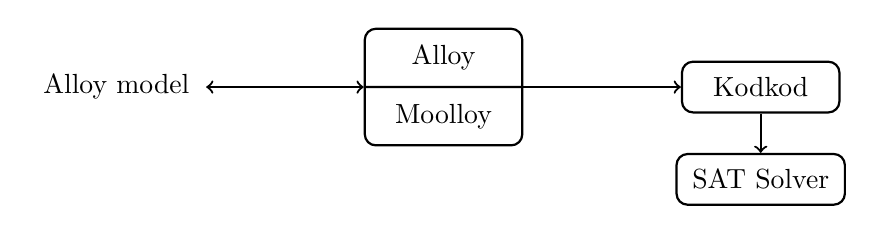
\begin{tikzpicture}[
      every node/.style={rectangle,thick,draw=black,text ragged,
                         rounded corners,inner sep=2mm,
                         text centered,minimum width=20mm},
      split/.style={rectangle split,rectangle split parts=2},
      double/.style={draw,thick,<->},
      single/.style={draw,thick,->},
    ]
      \node[draw=none] (model) {Alloy model};
      \node[split, right=2cm of model] (alloy) {
        \nodepart{one} Alloy
        \nodepart{two} Moolloy
      };
      \node[right=2cm of alloy] (kodkod) {Kodkod};
      \node[below=0.5cm of kodkod] (sat) {SAT Solver};
      \path(model) edge[double] (alloy);
      \path(alloy) edge[single] (kodkod);
      \path(kodkod) edge[single] (sat);
    \end{tikzpicture}
  \caption{Overview of Moolloy structure.}
\end{figure}

%\subsection{Product Perspective}
% Describe the environment of the system
% Include a context diagram
% A detailed description is not necessary since interface
% specifications appear later
% This section includes requirements of the user interface, such as
% testable usability requirements

Moolloy, as an extension of Alloy, is written in Java. It is backed by
Kodkod, which in turn makes calls to an external SAT solver. Kodkod and
the SAT solver are packaged with Moolloy.

%\subsection{Product Functions}
% Overview of system's main features
% Need give only a textual list of UC names

As input, Moolloy takes a multi-objective optimization problem modelled
in Alloy, and returns the Pareto front as an Alloy instance.

%\subsection{User Characteristics}
% Document any assumptions you make about the user and any assumptions
% you make about the background or how much training the user will need
% to use the system
% Consider only characteristics that affect the software requirements

We assume that all users are already familiar with multi-objective
optimization, including such terms as \textit{Pareto-optimal} and
\textit{Pareto front}. Furthermore, we assume users are familiar with
how SAT solvers are used to find these solutions. The user should also
be familiar with expressing the problem in Moolloy's domain specific
language, as well as interpreting the results.

%\subsection{General Constraints}
% Other constraints

%\subsection{Assumptions and Dependencies}
% Assumptions about input/environmental behaviour
% e.g. hardware never fails, ATM casing is impenetrable

As Moolloy is implemented in Java, the user will need to have the Java
Runtime installed on his or her environment.

%%%%%%%%%%%%%%%%%%%%%%%%%%%%%%%%%%%%%%%%%%%%%%%%%%%%%%%%%%%%%%%%%%%%%%
\section{Specific Requirements}\label{sec:specific_reqs}
% Requirements and specifications
% UML and UI diagrams go in here

\subsection{External Interfaces}\label{sec:ext_int}
% Detailed descriptions of all inputs and outputs
%     Name of input (or output)
%     Description of purpose
%     Source of input or destination of output
%     Valid range, accuracy, and/or tolerance
%     Command formats

Moolloy takes in various command-line arguments as input parameters.
Input problems are specified as Alloy models, while solutions are
output as Alloy instances.

\subsubsection{Command-line arguments}\label{sec:cl_args}

Moolloy has the following command-line arguments:

\begin{itemize}
  \item \verb|--SingleSolutionPerParetoPoint, -s|\\
  These two equivalent options specify that only a single solution is
  computed for each Pareto point. Defaults to False.

  %\item \verb|--ListOnlyOneSolution|\\
  %Specifies that only one solution is computed. Defaults to False.

  \item \verb|--LogRunningTimesArg=filename|\\
  Enables logging of running times to a file. Output will be written to the
  file \texttt{filename}. Defaults to False.

  \item \verb|--NoAdaptableImprovement|\\
  This option specifies that no adaptable minimum improvement at each
  step should be used. Defaults to False.

  \item \verb|--LogPrintHeaders|\\
  This option outputs the header in the log. Defaults to False.
\end{itemize}

Additional command-line arguments may be added to the external
interface to control optimization parameters. For example, flags may
selectively enable optimization features. Because this is a research
project and we do not know which techniques will be implemented, we
cannot concretely specify the arguments at this time.

\subsubsection{Input model}\label{sec:in_model}

The input model, specified as an Alloy file, is passed to Moolloy as
the last command-line argument. The file follows the Alloy
grammar~\cite{ref:alloy_grammar}, with a few Moolloy specific additions
to allow the definition of objectives and to run the corresponding
optimizations. Objective blocks are supported to define a series of
metrics and whether they should be maximized or minimized. Inst blocks
are also available to allow the creation of a set of typescopes which
can be referred to in the run command as the bounds of the
configuration space. This new bounds block can be referenced wherever a
typescope is required.

\begin{verbatim}
Additions to existing grammar rules
    paragraph ::= objectiveDecl
    typescope ::= name
    cmdDecl ::= [name ":"] ["run"|"check"] [name|block]
                scope "optimize" name

Objective Declaration
    objectiveDecl ::= "objective" name
                      "{" metric ["," metric] "}"
    metric ::= ["maximize"|"minimize"] name

Inst Declaration
    instDecl ::= "inst" name "{" typescope ["," typescope] "}"
\end{verbatim}

For examples of Moolloy input files see the test cases provided in
our test plan document.

\subsubsection{Output instance}\label{sec:out_model}

Moolloy returns the solution as an Alloy instance. Alloy instances are
expressed as XML files. In this case, solutions are generated as files
with the name \texttt{alloy\_solutions\_N.xml} where \texttt{N} is the
solution number.

TODO: What is the grammar/format of this XML file?

\subsection{Functional Requirements}\label{sec:func_req}
% Organize by features
%     Use case descriptions
%     Sequence diagrams
%     Domain model
%     Functional specifications
%     State machine model
%     Constraints

Moolloy takes in a multi-objective optimization problem as an Alloy
model, a format described in Section~\ref{sec:in_model}. It applies the
guided improvement algorithm to compute the Pareto front of the
specified problem. These solutions are converted to an Alloy instance,
expressed as XML, as described in Section~\ref{sec:out_model}.

If the \texttt{SingleSolutionPerParetoPoint} flag is specified, then
Molloy will compute only one solution for each Pareto point. If this
flag is not specified, Moolloy will use its default settings, which
will return all solutions that result in that Pareto point.

If the \texttt{LogRunningTimesArg} flag is specified, then Molloy will
log running times to the specified file. By default, this flag is not
set.

If the \texttt{NoAdaptableImprovement} flag is specified, then Moolloy
will not use the adaptable improvement optimization, which was exists
in the original version of Moolloy. This optimization uses exponential
steps when searching for better solutions. By default, this flag is not
set.

If the \texttt{LogPrintHeaders} flag is specified, then Moolloy will
include column headers in the log files. By default, this flag is not
set.

\subsection{Performance Requirements}\label{sec:perf_req}
% Stated in concrete terms

We are concerned with two performance requirements: speed and
scalability. These two are related, as significant improvements in
speed will allow Moollloy to scale up and handle larger inputs.

\subsubsection{Speed}\label{sec:perf_speed}

Moolloy's algorithm works by making multiple calls to a SAT solver for
each multi-objective problem it must solve. These calls can be
classified as \textsc{sat} and \textsc{unsat} calls, where \textsc{sat}
calls can be satisfied, and \textsc{unsat} calls cannot be satisfied.
\textsc{unsat} calls are very expensive, while \textsc{sat} calls are
less expensive, since they terminate once a solution is found.

Our goal is to improve the speed at which Moolloy solves a problem.
This allows users to solve our current problems much faster. To
accomplish this goal, we aim to reduce the number of \textsc{sat} and
\textsc{unsat} calls.

From Rayside et al.'s paper~\cite{ref:Rayside09}, the twenty-five
variable, four metric knapsack problem takes approximately forty-five
hours to complete, in the process requiring 1,938 calls to the SAT
solver, where 814 were \textsc{unsat}. Our goal is to reduce this time
to under twenty-four hours.

\subsubsection{Scalability}\label{sec:perf_scale}

Because solving large problems is very expensive, there are many
real-world problems that simply cannot be solved at this time. We aim
to optimize Moolloy so that such problems are solvable.

\subsection{Design Constraints}\label{sec:constraints}

As Moolloy is currently implemented in Java, the new version must also
be implemented in Java. Furthermore, to maximize the utility of this
program, Moolloy must be able to build and run on any platform that
supports Java.

%%%%%%%%%%%%%%%%%%%%%%%%%%%%%%%%%%%%%%%%%%%%%%%%%%%%%%%%%%%%%%%%%%%%%%
%\section{Current Implementation Details}\label{sec:impl}

% Appendices
% Index

\printbibliography[heading=bibintoc]

\end{document}
